\documentclass[a4paper,12pt]{article}

\usepackage{graphicx}
\usepackage{algorithm}
\usepackage{algorithmic}
\usepackage{amsmath}
\usepackage[usenames,dvipsnames]{color}
\usepackage{listings}

\definecolor{Brown}{cmyk}{0,0.81,1,0.60}
\definecolor{OliveGreen}{cmyk}{0.64,0,0.95,0.40}
\definecolor{CadetBlue}{cmyk}{0.62,0.57,0.23,0}
\definecolor{orange}{rgb}{0.7,0.3,0}
\definecolor{graycolor}{rgb}{0.2,0.2,0.2}
\definecolor{lightlightgray}{gray}{0.9}

\lstset{
language=C,                             % Code langugage
basicstyle=\ttfamily,                   % Code font, Examples: \footnotesize, \ttfamily
keywordstyle=\color{OliveGreen},        % Keywords font ('*' = uppercase)
commentstyle=\color{graycolor},              % Comments font
stringstyle=\color{orange},
numbers=left,                           % Line nums position
numberstyle=\tiny,                      % Line-numbers fonts
stepnumber=1,                           % Step between two line-numbers
numbersep=5pt,                          % How far are line-numbers from code
backgroundcolor=\color{lightlightgray}, % Choose background color
frame=none,                             % A frame around the code
tabsize=2,                              % Default tab size
captionpos=b,                           % Caption-position = bottom
breaklines=true,                        % Automatic line breaking?
breakatwhitespace=false,                % Automatic breaks only at whitespace?
showspaces=false,                       % Dont make spaces visible
showtabs=false,                         % Dont make tabls visible
morekeywords={__global__, __device__, __global, __kernel},  % CUDA specific keywords
}


\begin{document}

\title{An efficient GPU framwork for Image Processing}
\author{Per Karlsson}
\date{September 2014}
\maketitle

\setlength\parindent{0pt}

\begin{abstract}
\noindent
To be added

\end{abstract}


\tableofcontents
\setcounter{tocdepth}{2}

\section{Introduction}
\subsection{Background}
\subsubsection{Image processing}
An image can be seen as a mathematical function $i(x,y)$ where $x$ and $y$ are the spatial coordinates and the output is a color at position $(x,y)$. If the color has a discrete quantities and the total image has a finite element of samples, it is called a \emph{Digital Image}. The samples each has a unique spatial coordinate and are referred to as \emph{pixels}. The field of \emph{Digital Image Processing} refers to processing a digital image and its pixels. Every time Image Processing is mentioned in this theis, it is assumed that it refers to Digital Image Processing. 
\newline

The most typical application in image processing is when an algorithm is used to create a modified output image from an input image. This can be operations such as blur, sharpen and noise removal, all common techniques in standard image editing software. Figure \ref{lena} shows and example of a blur operation.
\begin{figure}[ht!]
\centering
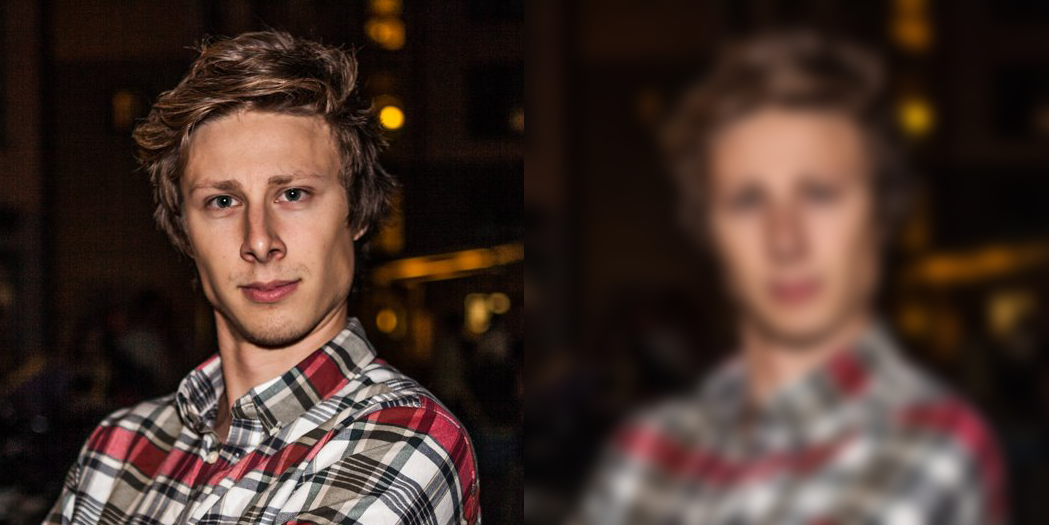
\includegraphics[width=80mm]{img/klas.png}
\caption{A blur algorithm is applied on an input image and produces a blurred output image.}
\label{lena}
\end{figure}

Another possible application would be where a function is used on an input image to extract information and features in the image. Figure \ref{feature} shows an example of a feature detection algorithm performed on an image containing a face. The algorithm manages to locate features such as nose, mouth and the eyes. Although the image is processed, not everyone agrees that this is typical application of image processing. Some people think this belong to the computer vision field. 

\begin{figure}[ht!]
\centering
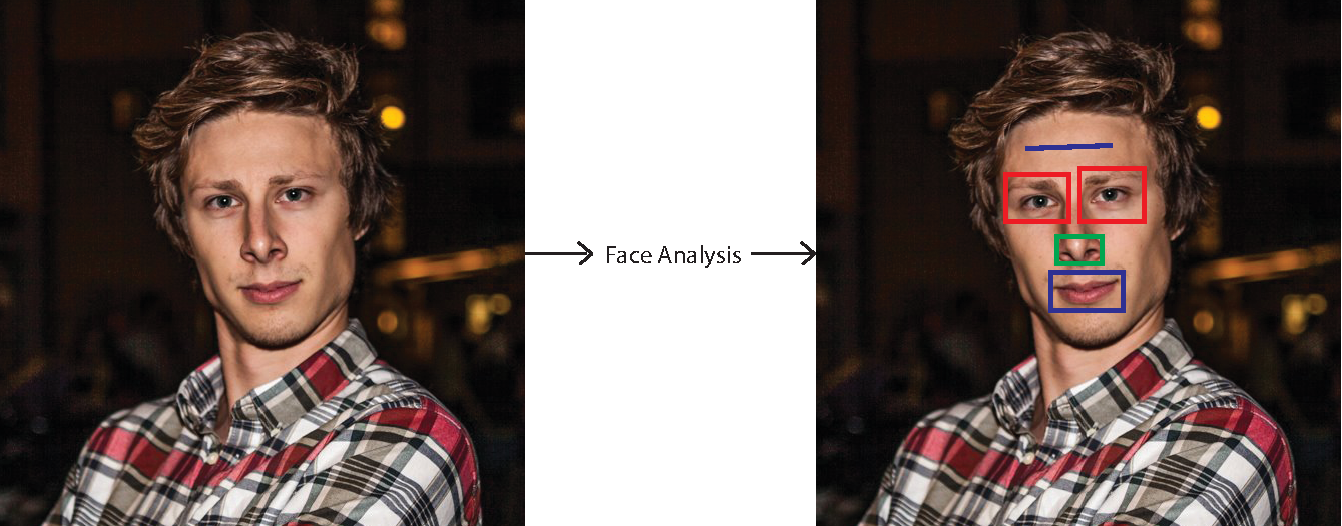
\includegraphics[width=80mm]{img/feature.pdf}
\caption{The input image of a face is analyzed to find features such as nose, mouth and eyes.}
\label{feature}
\end{figure}

\subsubsection{The evolution of computing hardware}

In the early 1960s, computers finally had enough computing power to perform meaningful image processing. The \emph{Jet Propulsion Laboratory} processed images of the moon captured by the on-board camera on the space probe \emph{Ranger 7} where they corrected image disortion. Later on, fields such as medical imaging astronomy started exploring the field of image processing. 
\newline

As the years passed by, the capacity of the computing hardware found in computers would keep improving. The term \emph{Moore's Law} was introduced based on a statement from the co-founder of Intel Corporation saying that the transistor count in integrated circuits are increasing by a factor of two every year. This was one of the reasons why the computing capability of processors kept increasing. The faster a processor's clock is operated, the faster a floating point computation is. In the early 1980s, the CPUs ran with internal clocks operating around 1 MHz. Today, around 30 years later, most CPUs have clock speeds around 2-4 GHz, which is a whole magnitude faster. Figure \ref{intelcpu} gives an overview of the transistor count and clock speeds of Intel CPUS the last 40 years.
\newline
\begin{figure}[ht!]
\centering
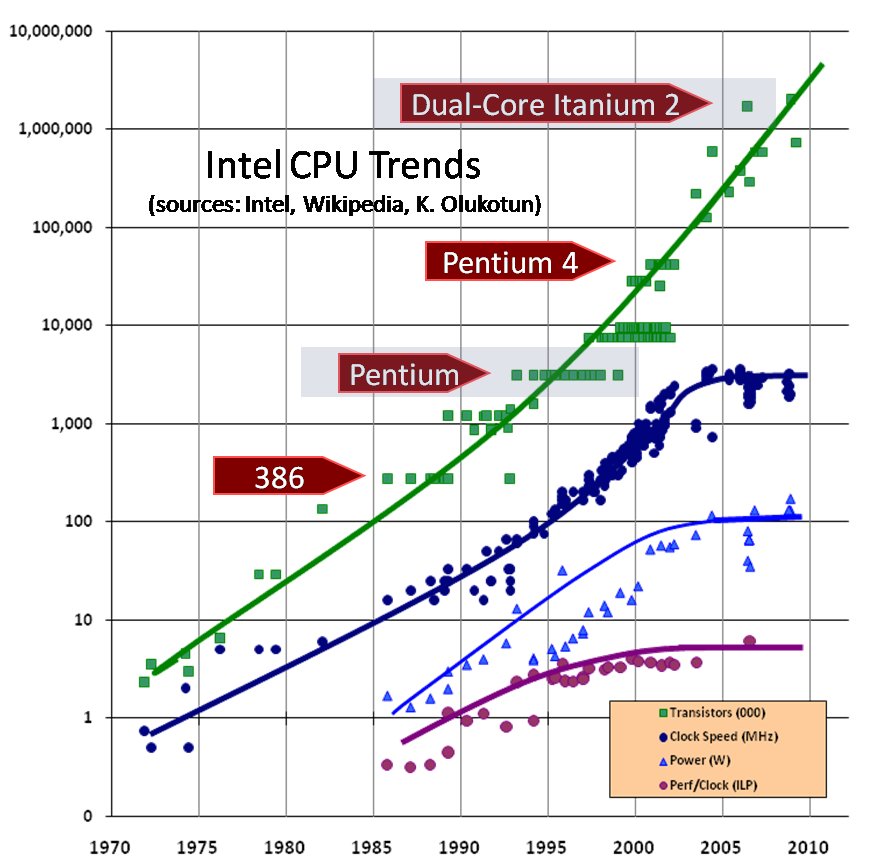
\includegraphics[width=70mm]{img/CPU.png}
\caption{The CPU transistor count has been growing exponentionally in the last 40 years.}
\label{intelcpu}
\end{figure}

Due to power and heat restrictions and the physical size of the current transistors, it is hard to keep improving the clock speeds. As of recent, the focus has shifted towards parallel computing and multicore processing units.

\subsubsection{GPU computing}

Computer games started became more popular in the 1990s. Computing was the big bottleneck in 3D graphics and it was hard to produce good real-time solutions. Therefore, companies started to experiment with a new computing device, the \emph{Graphical Processor Unit}, GPU. Instead of doing everything on the CPU, lighting computations and transforms of 3D coordinates could now entirely be done on the GPU. Since the computations of each pixels could be calculated independently of the others, it motivated the use of parallelism. 

\begin{figure}[ht!]
\centering
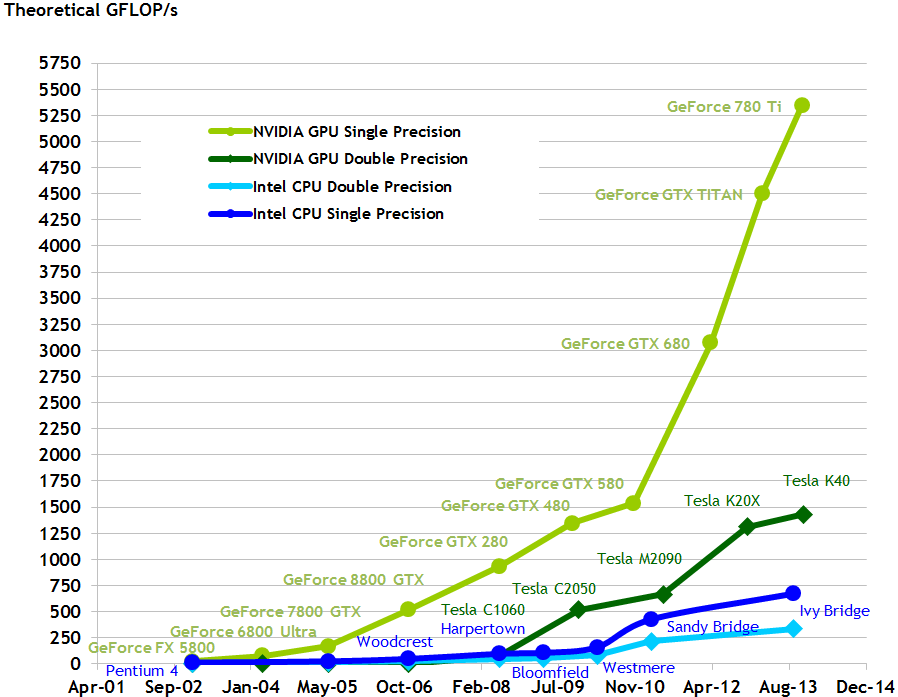
\includegraphics[width=90mm]{img/flops.png}
\caption{A comparison of theoretical floating point operations per second between CPUs and GPUs.}
\label{flops}
\end{figure}

When a GPU uses its full power and all computing units are used to maximum efficiency, a GPU is a lot faster than a CPU in terms of floating point operations per second. Figure \ref{flops} shows a comparison between the most recent CPUs and GPUs. The reason why the GPU is has lot higher theoretical maximu is because it is specalized for compute-intensive and highly parallel computations. It is therefore designed in a way that more transistors are devoted for data processing rather than data caching and flow control (which a CPU handles a lot better). 

\subsection{Purpose}

Most image processing tasks are well-suited for parallel computing. The average image consists of millions of individual pixels. This is a good case for GPU computing where a lot of the compute units can be utilized at the same time. To get started with GPU computing, one has to choose a parallel GPU environment to write the code in. There are different environments available, each with its own pros and cons. Which one to choose can sometimes be difficult to decide since it requires testing. In some cases, it might not be clear which environment is the best overall since they all have unique subfeatures.
\newline

GPU computing can be split into two steps. The first step is the configuration phase where the GPU environment is instantiated, memory is allocated on the GPU, data is copied to the GPU and the image processing code is compiled to GPU machine code. The configurations vary from environment to enviroment and it can be tedious to do this setup in every program with GPU computing. This motivates the use of a framework for efficient image processing on the GPU. This thesis will focus on implementing this framework, supporting the common GPU environments. It will try explore and hopefully answer the following questions:
\newline

\begin{itemize}
\item{What do the common GPU architectures have in common?}
\item{How do you generalize GPU computing for image processing?}
\item{Is it possible to write one functional framework although the environments and their architectures are different?}
\item{What restrictions have to be made?}
\item{Is it worth doing image processing on the GPU instead of the CPU?}
\end{itemize}

The second part of GPU computing is implementing the actual algorithms that run on the GPU. This part is hard to generalize since every GPU environment has its own coding language and special features. 
\newline

The work of this thesis will result in three different software components. They are the following:

\begin{enumerate}
\item{\bf{General backend framework}}
\begin{itemize}
\item{C++ library}
\item{Cross-platform}
\item{Easy to disable components from compilation}
\item{Possible to dynamically rebuild GPU code at runtime}
\item{Support python bindings}
\item{Unit tests for all implementations and cases}
\end{itemize}

\item{\bf{Graphical User Interface application}}
\begin{itemize}
\item{Python}
\item{Graphical display of the image outputs}
\item{Quickly change parameter values}
\item{Support for live coding}
\item{Save an algorithm setup for later use, including code and parameters}
\end{itemize}

\item{\bf{Command-line application}}
\begin{itemize}
\item{Python}
\item{Run the algorithm setup saved from the GUI-version}
\item{Change parameter values through command-line arguments.}
\end{itemize}
\end{enumerate}

\subsection{Limitations}

As discussed in the previous chapter, there are different categories in image processing. This thesis will focus on the case where an input image is used to produce an output image, mainly because it is hard to generalize things like feature extraction across all GPU environments. The framework is instead going to support algorithms where an arbitrary number of input images are going to produce an arbitrary number of output images. The number of input images and output images do not have to match. The framework needs to support multipass algorithms where multiple GPU programs are being called sequentially and where the output of one program can be the input of the following one. The framework is going support images with one to four channels of colors and where the data has either floating point precision or is of the unsigned byte type (often referred to as unsigned char).
\newline

The framework is going to support the following common GPU computing environments:

\begin{itemize}
\item{{\bf CUDA} - NVIDIA}
\item{{\bf OpenCL} - Khronos Group}
\item{{\bf GLSL} - OpenGL Shading Language}
\end{itemize}

CUDA and OpenCL are the two most common choices today in the world of general-purpose GPU computing. Before OpenCL and CUDA, people used programmable shaders in 3D graphics libraries such as OpenGL and DirectX to perform image processing on the GPU. Since DirectX and their HLSL shading language and Direct Compute environment only are supported on Microsoft Windows systems, they are not included in the framework of this thesis. The framework is meant to be flexible and cross-platform, supporting Unix, Mac OSX and Windows operating systems.

\subsection{Method}

The first phase of the thesis work will involved individual work with CUDA, OpenCL and GLSL to gain more knowledge about the different GPU environments. The middle phase of the project was the implementation of all the software components. This was be an iterative process. First a prototype was be created and after feedback from a supervisor and other people involved in the project, a second improved version was be implemented. For every feature added in the backend library, a unit test was added to test the different cases. The last part of the thesis work involved testing and more specifically, testing with practical image processing problems. The testing part served the purpose of benchmarking performance, testing how practical the framework is and examined if any GPU environment is better than the others in terms of functionality.

%\subsection{Structure}
This thesis is going to be structed the following way:

\begin{itemize}
\item{\bf{Introduction}}
\item{\bf{Parallel Environments}}
\item{\bf{Implementation}}
\item{\bf{Test cases}}
\item{\bf{Result}}
\item{\bf{Discussion}}
\end{itemize}




\section{GPU Environments}
\subsection{GLSL}

\subsubsection{OpenGL}

OpenGL is a cross-platform API that has been an industry-standard ever since it was introduced in 1992. Major decisions are made by the OpenGL Architecture Review Board, ARB. ARB was created by Silicon Graphics in 1992 and contained representatives from SGI, Intel, Microsoft, Compaq, Digital Equipment Corporation, Evans \& Sutherland and IBM. Later on, companies such as 3Dlabs, Apple, ATI, Dell, IBM, Intel, nVIDIA and Sun Microsystems were added. OpenGL shares many characteristics of a previous API called Iris GL. It is designed in a way where it tries to be the lowest level interface for accessing graphics hardware but still provide hardware independence. OpenGL is supported in PC, Mac and Unix-systems.

\begin{figure}[ht!]
\centering
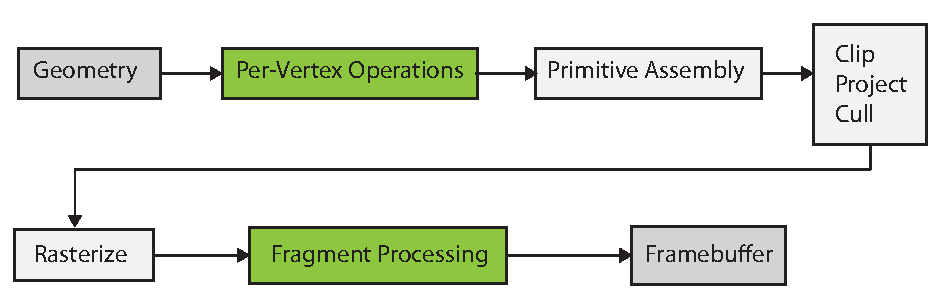
\includegraphics[width=100mm]{img/glpipeline.pdf}
\caption{OpenGL orginially had a fixed pipeline where non of these steps could be modified.}
\label{glfixed}
\end{figure}

Figure \ref{glfixed} shows the overview of the complete OpenGL pipeline in version 1.5 and earlier. It was said to have fixed functionality because every OpenGL implementation was required to have the same functionality. The set of operations and how they were applied were defined by the fixed OpenGL specification. The Fragment Processing step in Figure \ref{glfixed} is where each fragment gets its final value. A fragment can be thought of as the data needed to both shade the pixel decide if the fragment is to be displayed as a pixel (need information about depth, alpha). The fixed fragment stage could only handle tasks such as interpolating color values, texture mapping and fog. 

\subsubsection{The shading language}

In version 2.0, OpenGL introduced GLSL, the OpenGL shading language. With the OpenGL shading language, the fixed functionality stages for vertex and fragment processing (green steps in Figure \ref{glfixed}) could now be customized and programmed. It was still possible to do everything that the previous fixed pipeline supported but it also gave the software developer the opportunity to alone control the output. The programs written in GLSL are called OpenGL shaders, vertex shaders or fragment shaders. The OpenGL Shading Language is a high-level procedural language based on C and C++ syntax and flow control. Vector and matrix types/operations is natively supported together with a set of  math functions commonly used in graphics shading.
\newline

\subsubsection{Shaders}

\begin{figure}[ht!]
\centering
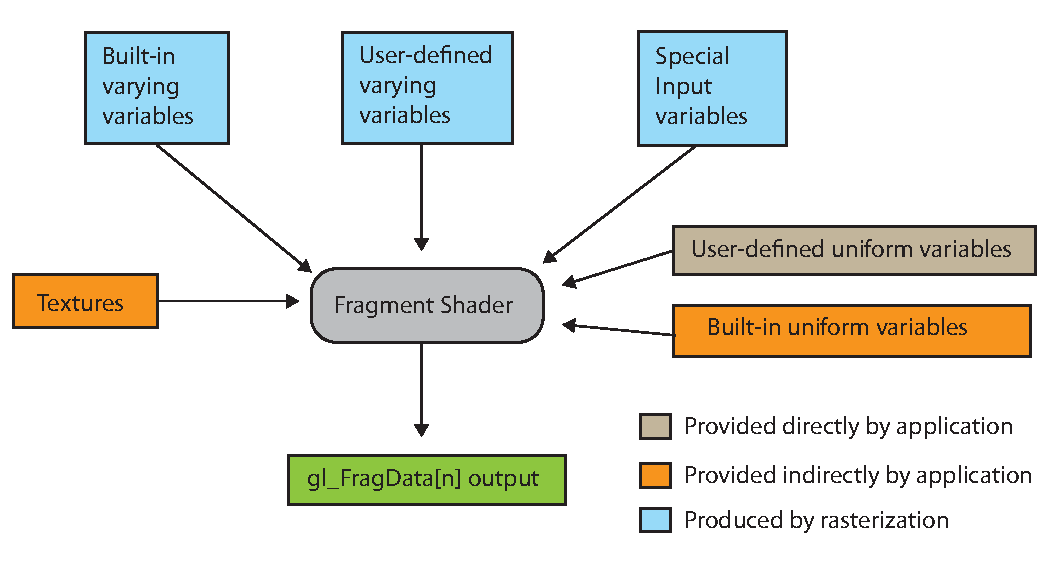
\includegraphics[width=100mm]{img/frag.pdf}
\caption{The inputs and outputs of a GLSL fragment shader.}
\label{glfrag}
\end{figure}

Shaders are compiled from an input source of text at runtime. They are later linked to an OpenGL program and become executable. In image processing, only the fragment shader is of importance. In a fragment shader, any image processing algorithm can be applied on an input image. A fragment shader operates on one fragment at a time. Fragment shaders must be written in such a way that they can operate simulationeusly. When a fragment shader is being executed, it has no knowledge about other fragments and their data. 
\newline

Figure \ref{glfrag} shows the inputs and outputs of a fragment processor. Some variables are built-in, specified by the OpenGL implementation. There is a notion of varying and uniform variables. Uniform variables are, as the name suggests, uniform across all shaders. Varying variables are defined per vertex in the vertex shader. Before processing each fragment, the hardware interpolates the geometry and gives the fragment shader the correct varying attributes. An example of a varying attribute is texture coordinates. The texture coordinates are defined at each vertex. Before the processing of the fragment shader, the texture coordinates are interpolated across the geometry and can be used later in the fragment shader to do texture lookups.

\renewcommand{\lstlistingname}{Code}
\begin{lstlisting}[caption= Example of adding two images in GLSL, label=glsl1]
uniform sampler2D texture0;
uniform sampler2D texture1;

uniform float scale;
varying vec2 texcoord;

void main()
{
    gl_FragData[0] = scale * (
        texture2D(texture0, texcoord) + 
        texture2D(texture1, texcoord));

}
\end{lstlisting}

Code \ref{glsl1} shows an example of fragment shader in GLSL that adds two images together. The images have been converted to OpenGL textures, \texttt{texture0} and \texttt{texture1}. The function \texttt{texture2D} together with the varying variable \texttt{texcoord} is used to fetch the data from a texture. The value is multiplied with the uniform value \texttt{scale} (same for all fragments) and finally written to the framebuffer through the built-in \texttt{gl\_FragData}. Syntax is similar to a C program and every fragment shader needs a \texttt{main} function.

\newpage
\subsection{CUDA}

The CUDA architechure was released for the first time in 2006 to make it easier to perform general purpose GPU-computing. Unlike previous methods that had to get around the old pipeline with vertex and fragment shaders, CUDA allowed every aritmethic logic unit on the chip to be controlled by a CUDA program. Another important feature was the possibility to read and write to arbitrary memory address on the GPU in comparison to previous methods that required textures as storage. The hardware was still in charge of memory caching but CUDA also exposed a software managed cache called shared memory. CUDA programs are written in the CUDA C language, a language very close to the C language with the exception of a small number of keywords added for special features in the CUDA architecture.  

\subsubsection{Blocks and threads}

In the CUDA architechure, threads are single execution units that run kernels on the GPU. They are similar to CPU threads but the typically there are a lot more of them on the GPU. The threads are divided into thread blocks. Threads within a thread block can communicate with each others. The number of blocks and threads per block is decided by the developer when the kernel is called. The grid of block can be one, two or three dimensional. The maximum number of blocks and threads per block is decided by the GPU and its hardware. A CUDA kernel is executed simulatenously by warps. A warp consists of threads within a block. Typically each warp has the size of 32 threads, where actions like memory read and writes are performed in half-warps. 
\newline

\begin{figure}[ht!]
\centering
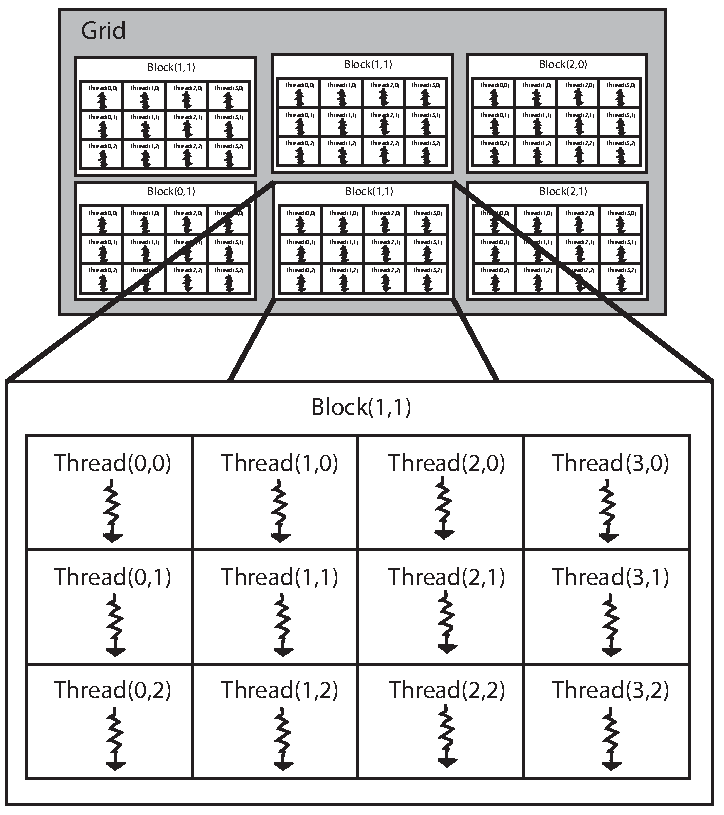
\includegraphics[width=80mm]{img/cuda.pdf}
\caption{CUDA threads divided into blocks of threads.}
\label{cudablockthreads}
\end{figure}

\renewcommand{\lstlistingname}{Code}
\begin{lstlisting}[caption= Example of vector addition in CUDA, label=cuda1]
__global__ void VectorAddition(float * A, 
                               float * B, 
                               float * C)
{
    int i = blockIdx.x * blockDim.x + threadIdx.x;
    int j = blockIdx.y * blockDim.y + threadIdx.y;
    int idx = i + j * gridDim.x * blockDim.x;
    C[idx] = A[idx] + B[idx];
}
\end{lstlisting}

When a thread is executing a kernel, there are built-in variables to access information of which block the thread belongs to and the local thread index in the actual block. This is often used to know where to read and write in a global array. Code \ref{cuda1} shows an example of a simple CUDA kernel performing a vector addition. The keyword \texttt{\_\_global\_\_} is used to tell the compiler that the function is a CUDA kernel. The variables \texttt{blockIdx}, \texttt{threadIdx}, \texttt{gridDim} and \texttt{blockDim} are automatically built-in in a CUDA kernel and can be accessed at any time. \texttt{blockIdx} and \texttt{threadIdx} are of the type \texttt{uint3}, where each value represent an index in the corresponding dimension. \texttt{blockIdx} is the index of the block in the total grid of launched blocks and \texttt{threadIdx} is the thread index within the block. Both \texttt{gridDim} and \texttt{blockDim} are of the type \texttt{dim3} and are constant in all threads (not possible to launch a kernel with different block sizes).

\subsubsection{Memory hierarchy}
\begin{figure}[ht!]
\centering
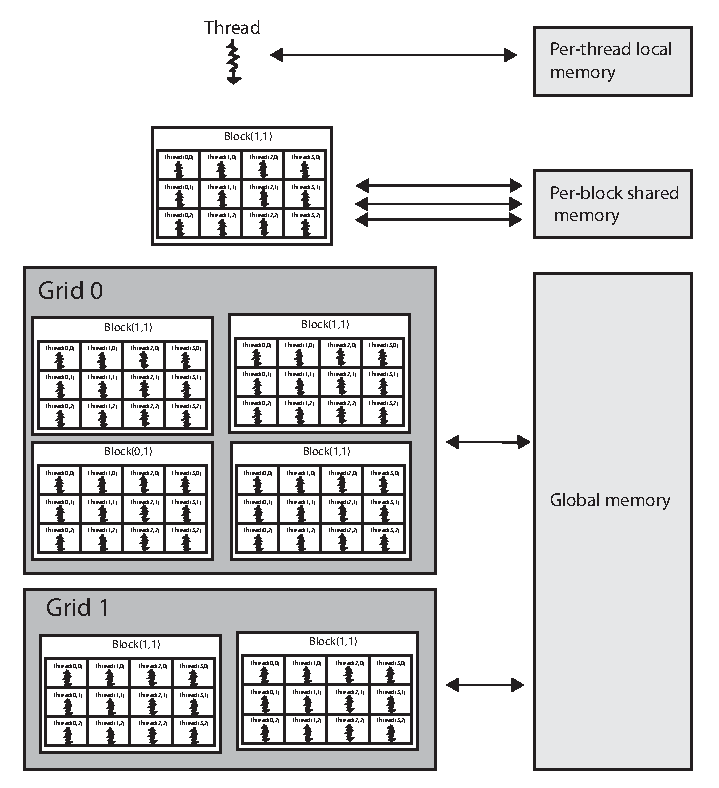
\includegraphics[]{img/cuda2.pdf}
\caption{Different CUDA memory spaces}
\label{cudamemoryhierarchy}
\end{figure}
There are differnet memory spaces in the CUDA architechure as can be seen in Figure \ref{cudamemoryhierarchy}. Each thread has a local and private memory space. All the threads in a block can share a memory space, called shared memory. Shared memory is on-chip and is divided into different banks. Reading from shared memory in warp of threads is just as fast as reading from a register as long as there are no bank conflicts. Each bank conflict results in a serialized read from the shared memory. Worst case scenario is when all threads in a warp only read from one bank in the shared memory. The shared memory read then becomes a lot slower then the regular global memory. Global, constant and texture memory can all all be accessed by all threads. Constant and texture memory are only used in certain cases where the global memory is the common choice for storing data. The texture memory space is cached to that a texture fetch only cost a GPU device memory read on a cache miss, otherwise it only costs a read from the texture cache. Texture cache is optimized for 2D spatial locality. If desired, one also gets an automatic linear interpolation when reading from the texture space. Constant memory is a read-only memory space. All the threads of a half-warp read from constant memory just as fast as from a register as long as all the threads read from the same address. The cost scales linearly with the number of different addressed read by the threads. For example, the worst case would be if an array would be stored in the constant memory space and each thread in an executing half-warp needs an unique value in this array. The commonly used global memory space is capable of reading 4, 8 and 16 bytes of memory into registers in one single instruction. The most efficient global memory reads are when all threads in a half-warp reads from continous memory in a coalesced read of 64, 128 or 256 bytes. It is impossible for a thread to know if the current value in the global memory  has been updated or not if a kernel is reading and writing to the same global memory. CUDA supports atomic operations but they are usually slow and a common technique is to have to different buffers allocated, one to read from and one to write to.




\subsection{OpenCL}

\subsubsection{Standarized framework for heterogeneous systems}

OpenCL is a parallel programming framework designed to fit heterogeneous systems where one can expect a range of different computing architechures. One example of a program on a heterogeneous system would be a program where some parts of the computations and setups are done on the CPU and the rest on the GPU. OpenCL also supports parallel programming for homogeneous systems. In a case where one has a multi-core CPU, OpenCL could be used to in such way to have one thread control the state of the program while the rest of the threads performs a computation of some sort and later sync with the main thread.
\newline

OpenCL is standarized by the Khronos Group, the same group in charge of well known OpenGL standarization. The group consits of people from many different companies in the industry such as AMD, nVIDIA, intel, Apple, Samsung. This is seen as a positive thing as they all decide the direction the group is taking. It also makes sure the framework compatible for different system and platforms. One of the goals of OpenCL is to be as flexible as possible.
\newline

\subsubsection{The OpenCL C language}
OpenCL can be used in any parallel environent as long as the OpenCL compiler and runtime library is implemented. This means, when writing the parallel code, a software developer do not have have care about operating system, processors and memory types. The OpenCL C language is very similar to the regular C language. It is focused around computations and some features are added on top of the C language to simplfy things, like SIMD vector operations and multiple memory hierarhies. Other features, such as printing, have been removed as they are not as useful in computing and hard to implement on all platforms. The program calling the OpenCL code can be written in either C or C++ as it will be using the OpenCL runtime library. 
\newline

The notion of host is often used in standard and offical OpenCL literature. The host refers to the environment where the OpenCL code is called from (not executed). This is the CPU in almost all of the cases. An OpenCL device is the environment where the OpenCL is executed. This can be the GPU, DSP, CELL/B.E, CPU are some examples of OpenCL devices that often contain a lot of small compute units each. The memory associated with these processors are also included in the defintion of an OpenCL device. The OpenCL code executed on a device is called \emph{kernel}.
\newline

\subsubsection{Memory Hierarchy}

Similar to the CUDA architechure, OpenCL also has a memory hierarchy. The OpenCL standard only specifices the access levels of the different memory spaces and there may be important performance details that are different on different hardware implementations. While it makes it possible to optimize the code for a certain hardware or vendor, it makes it harder to generalize and write programs with high performance accross different devices. 

\begin{figure}[ht!]
\centering
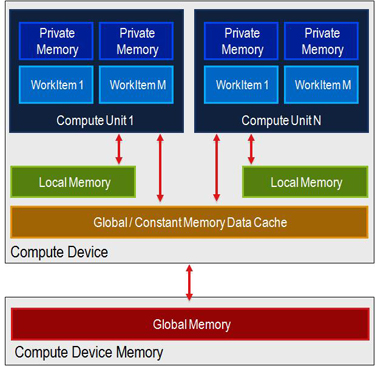
\includegraphics[width=70mm]{img/mem-cl.jpg}
\caption{OpenCL memory hierarchy.}
\label{cl-mem}
\end{figure}

\begin{itemize}
\item{{\bf Global Memory} - The global memory has the larget capacity and can be used by all work items. It is considered of being the slowest memory subsystem. The best performance is achieved when streaming contiguous memory addresses or patterns that can explore the full bandwidth (similar to the coalesced memory reads in CUDA). }
\item{{\bf Private Memory} - The memory used in a single work items. Can not be shared between work items. Similar to registers in GPU multiprocessors or CPU cores. The private memory is allocated and partioned at compile time. There is no maximum private memory size defined  in the OpenCL specification. Using too much private memory can lead to a slowdown since OpenCL will user slower memory spaces once the private memory is full.}
\item{{\bf Local Memory} - Local memory can be shared between work items in a work group, similar to the shared memory in the CUDA architechure. Local memory is used when data from global memory is needed and one wants to reduce the global memory reads within a work group.}
\item{{\bf Constant Memory} - Constant memory is implemented differently on certain deviced. For example, on NVIDIA GPU cards, the constant memory is located at region good for broadcasting. On ATI GPU cards, the constant memory is part of the global memory but with optimized broadcasting.}
\end{itemize}

\subsubsection{Work Groups}

Kernels are being executed over a 1D, 2D, 3D grid or NDRange. The kernel is then executed in parallel where each kernel instance is called work item. Work items are divided in work groups of the global grid. The developer can explicity set the size of the work group or let it be decided at runtime.

\renewcommand{\lstlistingname}{Code}
\begin{lstlisting}[caption= Example of vector addition in OpenCL, label=cl1]
__kernel void VectorAddition( __global float * A,
                              __global float * B,
                              __global float * C,
                              int width)
{ 
    const int x = get_global_id(0); 
    const int y = get_global_id(1); 
    const int idx = x + y * width;
    C[idx] = A[idx] + B[idx];
}
\end{lstlisting}

Code \ref{cl1} shows an example of a simple vector addition. Keyword \texttt{\_\_kernel} tells the compiler it is a OpenCL kernel and \texttt{\_\_global} specifices a pointer to the global memory space. Inside the kernel, the function \texttt{get\_global\_id} is used to find the horizontal and vertical id of the work item (this only works if the kernels are executed with a two dimensional work size).


\section{Implementation}
\subsection {Designing the core library}

On an abstract level, the workflows in the GPU environemnts are more or less the same. This motivates the use of a library where a developer can target a common abstract interface and not have to worry about specific GPU environment implementations. The library is named \emph{gpuip} which stands for \emph {GPU Image Processing}. The core superclass in \emph{gpuip} is called {\tt ImageProcessor} and it is through this class that all the GPU communication is going to happen. An implementation of an {\tt ImageProcessor} needs to support the following common steps:

\begin{enumerate}
\item Compile kernel text code and build into GPU machine code.
\item Allocate memory on the GPU.
\item Copy data from CPU to GPU and vice versa.
\item Run kernels on the GPU.
\end{enumerate}

These steps are all virtual functions in the {\tt ImageProcessor} class that needs to be implemented in the subclasses. The class {\tt Buffer} provides memory allocation information to {\tt ImageProcessor}. An algorithm can have an arbitrary amount of buffers. The input and outputs are stored in buffers. Each buffer has a unique name and information about data type and how many channels there are per pixel. The supported data formats are {\tt unsigned byte, half} and {\tt float}. {\tt half} is a 16-bit floating point scalar in comparison to the standard 32-bit {\tt float}. Each buffer can have between one to four channels per pixel. Two or three channels per pixels is supported but not recommended as it leads to uncoalesced reads and writes[ref]. 
\newline
\renewcommand{\lstlistingname}{Code}
\begin{lstlisting}[caption= Buffer struct, label=bufferapi]
struct Buffer{
    typedef shared_ptr<Buffer> Ptr;
    enum Type { UNSIGNED_BYTE, HALF, FLOAT };
    const string name;
    Type type;
    unsigned int channels;
};
\end{lstlisting}
\newpage
The {\tt Kernel} class provides the following:
\begin{enumerate}
\item GPU kernel code. Syntax and program structure depends on GPU environment.
\item Which buffers are going to be used as input? What are they called in the kernels?
\item Which buffers are going to have data written to them?
\item Parameters used in the kernel code.
\end{enumerate}

\renewcommand{\lstlistingname}{Code}
\begin{lstlisting}[caption= Kernel struct, label=kernelapi]
struct Kernel {
    struct BufferLink {
        Buffer::Ptr buffer;
        string name;
    };
    typedef shared_ptr<Kernel> Ptr;
    const string name;
    string code;
    vector<BufferLink> inBuffers;
    vector<BufferLink> outBuffers;
    vector<Parameter> params;
};
\end{lstlisting}

As can been seen in Code \ref{bufferapi} and Code \ref{kernelapi}, both structs have a {\tt Ptr} typedef. A {\tt Buffer::Ptr} is a shared pointer[ref] to a {\tt Buffer} object. To register a {\tt Buffer} or a {\tt Kernel} to an {\tt ImageProcessor} object, the factory method pattern[ref] is used. An example of this can be seen in Code \ref{factoryfunc}.
\newline
\renewcommand{\lstlistingname}{Code}
\begin{lstlisting}[caption= Factory functions to create Buffer and Kernel objects, label=factoryfunc]
class ImageProcessor {
    ... rest of ImageProccessor definitions ...

    Buffer::Ptr CreateBuffer(const string & name,
                             Buffer::Type type,
                             unsigned int channels);

    Kernel::Ptr CreateKernel(const string & name);
};
\end{lstlisting}
In this case, the factory method pattern guarantees that the {\tt ImageProcessor} is the \emph{owner} of the buffers and kernel objects since it is going to store a copy of the shared pointer internally. As long as the {\tt ImageProcessor} exists, the {\tt Buffer} and {\tt Kernel} objects are also guaranteed to exist. This makes it impossible to reach cases where the {\tt ImageProcessor} is using pointers that are pointing to deleted objects and is considered a safe approach. Anyone using the library can still create and delete {\tt Buffer} and {\tt Kernel} objects on their own, but they will never be able to register these objects themselves.

To make things simple, all GPU operations are synchronous which means that once a function that communicates with the GPU has been been called, it is not going to return until the GPU is done proceeding the task. There are asynchronous ways of calling the GPU in all environment but they require syncing stages. As discussed in [ref], it might be worth supporting asynchronous calls in the future since they could potentially give better performance.
\newline
\renewcommand{\lstlistingname}{Code}
\begin{lstlisting}[caption= {\tt ImageProcessor} API for GPU operations, label=ipapi]
class ImageProcessor {
    ... rest of ImageProccessor definitions ...

    virtual double Allocate(string * error);
    virtual double Build(string * error);
    virtual double Run(string * error);
    virtual double Copy(Buffer::Ptr buffer,
                        CopyOperationEnum operation,
                        void * data,
                        string * error);
};
\end{lstlisting}

As can be seen in Code \ref{ipapi}, all functions that perform GPU operations returns the execution time as a {\tt double} and takes a pointer to an error {\tt string}. If an error occurs inside one of these functions, a \emph{negative} value is returned and the error message can be found in the error string. 


\subsection{Implementing the subclasses}
\subsubsection{GLSL}
The user-provided kernel code is a fragment shader. To build a GLSL program, one also needs to provide a vertex shader. The built-in vertex shader in gpuip is simple and draws a 2D quad across the viewport, covering all pixels, and defines texture coordinates in each corner. These texture coordinates, as mentioned in Chapter 2.1, will be interpolated across all fragments. Since all fragment shaders use the same vertex shader code, it is compiled once and shared between all fragment shaders.
\newline

For each buffer, an OpenGL texture is generated and memory is allocated on the GPU. For each kernel, a framebuffer object is created. Depending on the kernel setup, every output buffer of a kernel is mapped the corresponding framebuffer object. This means that later on when the simple quad is drawn, the data is rendered to the textures directly. To copy data from and to the GPU, the synchronous functions {\tt glGetTexImage} and {\tt glTexImage2D} are used.
\newline

The input textures (buffers) and parameters has to be set before the GPU kernel code can be executed. Each uniform attribute has a location in the GLSL program. To get the location, {\tt glGetUniformLocation} is used. It is important that the input textures and parameters in the kernel code are named the same as the {\tt Kernel::BufferLink::name} and {\tt Kernel::params}, otherwise the GPU code will not run. Before calling the draw functions, the viewport has to be resized to the same resolution as the output buffers. The GPU calls are synchronized with {\tt glFinish} and timings are queried with {\tt glGetInteger64v} and {\tt GL\_TIMESTAMP}.

\subsubsection{OpenCL}

OpenCL needs a context for saving states and an event queue to register GPU operations in. Allocating memory is done through OpenCL buffers and kernel code is compiled at runtime with the standard OpenCL API calls {\tt clCreateProgramWithSource}, {\tt clBuildProgram} and {\tt clCreateKernel}.
\newline

When executing the kernel code, the kernel arguments have to be passed in the same order as they are presented in the kernel function. Kernel arguments include pointers to input and output buffers, user-defined parameters and gpuip parameters. Since the C++ code is bound to compile time and the kernel code is written at runetime,  there have to be rules that decides which order arguments appear in. The current ordering rules are:

\begin{enumerate}
\item {\tt const} pointers to input buffers
\item Pointers to output buffers
\item User-defined arguments
\item Gpuip-arguments (like image width and image height)
\end{enumerate}

Launching the kernels can only be done asynchronously. To guarantee that all GPU computation is done when the function returns, the OpenCL state is synced with {\tt clFinish}. Timings are captured with the {\tt clGetEventProfilingInfo}.

\subsubsection{CUDA}

Unfortunately, CUDA does not support compilation of GPU code at runtime which was one of the goals of gpuip. However, it does support loading of ptx, parallel thread execution, at runtime. Ptx is a pseudo-assembly language used by NVIDIA on the GPU. To get ptx files, we must use the NVIDIA-provided CUDA compiler \emph{nvcc}. Nvcc is called by {\tt popen} ( {\tt \_popen} on windows) which creates a pipe and invokes a shell command. When closing the pipe with {\tt pclose}, the exit status of nvcc can be queried. If the exit status is anything other than zero, the compilation failed and the error string can be read from the pipe.
\newline

CUDA comes with a driver API and a runtime API. The runtime API is user-friendly and the driver API gives more control. They can both be used at the same time. Loading compiled ptx files and execution of kernel calls are done through the driver API and the runtime API is used for context creation, memory allocation and data transfer. Allocating memory on the GPU is straightforward with the {\tt cudaMalloc} function, which is very similar to the C version {\tt malloc}. Copying data is also simple with {\tt cudaMemcpy}.
\newline

CUDA kernels are executed in blocks with a fixed amount of threads per block. In gpuip, every block consists of 256 threads distributed in a 16x16 thread-block. To make sure every thread corresponds to one pixel, we use the following equations to determine the number of blocks $N_x$ and $N_y$:

\begin{equation}
N_x = floor(W/16) + 1 ,\ 
N_y = floor(H/16) + 1
\end{equation}

where $W$ is the image width in pixels and $H$ is the image height. Some threads will have $xy$-coordinates outside of the image domain. To avoid writing to non-allocated memory, all threads need to check if they are inside the image domain.




\subsection{Python bindings}

Boost python [ref] is used to make the C++ code accessible in a python environment. When copying data from and to the GPU, one has to pass a void pointer in the gpuip C++ API. The concept of pointers does not exist in python. Instead, in the python bindings, the CPU data is attached to the buffer itself using a numpy [array]. All the data transfers between GPU buffers have to go through the numpy array.
\newline

A common task in image processing is to read image data from disk and later on write to disk once the processing is done. To simpify this step, read and write functions are included in the python bindings. Depending on the per element data in the numpy array, different file formats are available. For {\tt half} and {\tt float} precision, the target format is OpenEXR by ILM[ref]. When the data consists of unsigned bytes, the more common image formats png, jpeg, tiff and tga are available through the header-only library CImg[ref].  

\subsection{Graphical user interface}

The graphical user interface application is written in python since it often means faster development iterations. To fit the cross-platform requirements, the UI framework Qt\cite{qt} is used. The core of Qt is written in C++ but there are python bindings available. Gpuip uses PySide\cite{pyside} since they are well documented and supported on the official Qt homepage. 
\newline

The application will be a {\tt QMainWindow}. Main windows in Qt support menus and toolbars. All the different components will be dock widgets. A dock widget is resizeable and can be detached to a solo window. The following components will be added as dock widgets:

\begin{enumerate}
\item Toolbar. Add menu items and toolbar items as {\tt QAction}. It is possible to bind an action to a hotkey.
\item Preview. Display the content of a buffer using {\tt QGLWidget}. Supports zoom and pan. If the image has floating point precision, a slider controlling the exposure is added. This is based on the same display algorithm as exrdisplay\cite{exrdisplay}.
\item Code. This is a {\tt QTextEdit} containing the kernel code. When building a kernel, gpuip reads the text from this widget.
\item Params. Per kernel setup with {\tt QComboBox} dropdown menus for buffer selection and editing parameter value with {\tt QSlider} and {\tt QLineEdit}.
\item Log. Output log for all commands using {\tt QTextBrowser}.
\end{enumerate}

\subsection{Cross-platform build}
\subsubsection{Generate build setup}
Every platform has their own way of compiling source code into binaries. On Unix systems, gcc and makefiles is the common option while on Windows systems most code is compiled with Microsoft Visual Studio. CMake is a cross-platform build system by Kitware[ref]. CMake controls the software compilation step using platform independent configuration files. Option variables and cached string values can be defined in the configuration files and later on be modified at either the command line version of cmake or the gui version. This makes CMake a very powerful tool to setup customizable builds. For example, in gpuip, one can easily disable the build of the python bindings if it is not needed. Another case could be if the compiling system does not have a NVIDIA GPU and want to build gpuip without CUDA support. Once all options are set, CMake generates either Unix Makefiles, Microsoft Visual Studio or other build setups that are already configured. This means all the include paths for header files have been set and linking to other libraries is taken care of.

\subsubsection{Library dependencies}
Gpuip and especially its python bindings part depends on other open source libraries. When the compiler is invoked, information about where these libraries are located has to be passed. These locations can be vary a lot in different setups and it is hard to come up with a solution that is going to work nicely across all platforms. Luckily, CMake has a nice feature called {\tt FindPackage} where it is possible to register scripts to find external libraries. The most common libraries and their {\tt FindPackage} script are shipped with CMake. Some of the libraries used by gpuip were not reconized by {\tt FindPackage} in CMake and scripts for finding them were added.
\newline

It can be annoying to prepare all the prequisites building a library that depends on a lot of other libraries. To simplify this step, gpuip tries to make the build process as smooth and out of the box as possible. If a third party library is missing and it is an open source library, it will try to download the missing library at compile time and build it. This can be done through the {\tt ExternalProject\_Add} feature in CMake where one specify the path to the git or svn repository where the open source code exists. It is also possible to specify specific configure, build and install command if the open source library does not use CMake as build system.

\subsubsection{Regression testing}
CMake comes with ctest, which is tool that can be used for testing the code after building it. Gpuip has three differnet tests: One testing the standard API calls in C++, One testing the standard API calls in the python bindings and one that compares performance of gpuip vs cpu implementations (both single and multi-threaded).

\subsubsection{Documentation}
An API documentation is generated at build time (if the option is enabled) with the help of Doxygen[ref]. Doxygen reads the comments of the header files and generates an html and reader-friendly version to publish online. 



\section{Results}

\section{Discussion}
\subsection{Comparison between the GPU environments}

All GPU environments have both their pros and cons. After working on the implementation of each GPU environment, these are the my summarized conclusions:

\begin{itemize}
\item OpenCL
\begin{description}
  \item[$+$] Supports runtime compilation.
  \item[$+$] Works on any GPU and any CPU.
  \item[$-$] Poor 16-bit floating point support.
  \item[$-$] Does not support templating.
\end{description}
\item CUDA
\begin{description}
  \item[$+$] Easy to use with runtime API.
  \item[$+$] Debugging tools.
  \item[$+$] Supports templating and operator overloading.
  \item[$-$] Does not support runtime compilation.
  \item[$-$] Only works on NVIDIA GPUs.
  \item[$-$] Poor 16-bit floating point support.
\end{description}
\item GLSL
\begin{description}
  \item[$+$] Works on any GPU. OpenGL is include in a lot of systems by default.
  \item[$+$] Supports runtime compilation.
  \item[$+$] Abstract way of dealing with data.
  \item[$+$] Display functionality for free.
  \item[$-$] Setup is not clean. Need to fake render a quad.
  \item[$-$] Can only write to one pixel at a time.
  \item[$-$] No local shared memory between work items.
\end{description}
\end{itemize}

If I had to pick only one GPU environment to use in a new application, I would choose OpenCL because it is very flexible and runs both on CPU and the GPU. GLSL would be an okay choice as long as the application is about image processing. GLSL should work out of the box on most systems and that makes it very easy to deploy the application to other parties. However, for more general purpose computing, GLSL quickly becomes bulky and requires a lot of tricks. Writing OpenCL and CUDA kernels is about the same and the setup in CUDA is actually easier than OpenCL. The limitation of NVIDIA-only GPUs is too big of a factor to me and if NVIDIA would make CUDA run on all GPUs, I think CUDA would increase a lot in popularity. All the tests in this thesis were very basic and there might be a possibility that CUDA is the best environment to use once you want to optimize further and really get the most out of the GPU.

\subsection{OpenGL interoperability}

Currently, if an image has been created/modified with gpuip and needs to be displayed, it first has to be copied back to the CPU and then uploaded back to the GPU for viewing. Both OpenCL and CUDA support OpenGL interoperability by mapping a GPU buffer to an OpenGL buffer. This means that data produced by OpenCL and CUDA can be used as an OpenGL texture without unnecessary transferring between the CPU and the GPU. Although more internal work, the public API for {\tt Buffer} would not change much:
\newline
\renewcommand{\lstlistingname}{Code}
\begin{lstlisting}[caption= gpuip OpenGL interoperability, label=glinter]
struct Buffer{
  // ... rest of Buffer declarations 
  bool glInteroperability;
  GLint glTexture;
};
\end{lstlisting}

I think this option would make the library more lucrative to use in applications that are using OpenGL for viewing graphics. One particular case I could see it being useful is in deferred rendering for realtime 3D graphics. Once geometry has been rendered to different textures, it might be faster to apply operations in OpenCL or CUDA than it is in GLSL (there is no support for sharing memory between execution threads in GLSL).

\subsection{Template kernels}

Consider a case where you only want to write one kernel file but support multiple fileformats. For GLSL, this is already true and quite practical. However, it is not possible in OpenCL and CUDA. CUDA supports templated functions. CUDA only supports {\tt half} storage and not computation and it is therefore not possible to template a function and have it work the same with {\tt half}, {\tt unsigned byte} and {\tt float}. In OpenCL, half computation is supported if the graphics drivers come with the {\tt cl\_khr\_fp16} extension. OpenCL does not support templates but since we parse the kernel code ourselves in gpuip, we could implement our own templating rules and generate one OpenCL kernel for every data type that gpuip supports. 

\subsection{Computations as input}

It is only possible to write data per pixel in gpuip. If an algorithm would require a global property of a buffer, like the maximum or average value, it would not be possible. For example, if someone wants to write a tone mapping algorithm, they might compute a tone mapping value per pixel and then use the average value of all pixels as input to a second step in the tone mapping. A kernel can have user-defined parameters but not parameters that depend on the output of a kernel. It might be nice to add an option to make it possible to use the computation of a buffer as input. To make things still fairly simple, it could be restricted to only allow computations of one-dimensional buffers. Then a computation could support operators such as min, max, median, avg and sum. Internally, gpuip would perform the GPU algorithms. For example, to get the minimum value of a one-dimensional buffer, it would have to run a reduce algorithm. It might be worth exploring the common libraries for the GPU computing. Using libraries like Boost Compute\cite{boostcompute} and Thrust\cite{cudathrust} would save time and probably have better performance.

\subsection{Work item distribution}

Some algorithms might be optimized further by allowing a work item/thread to write to more than one pixel. For example, in separable blur algorithms, it might be worth splitting the algorithm in two steps and have each work item operate on a row/column alone. Memory lookups tend to be the expensive part of an algorithm and if a work item can work alone on a row, data could be stored in the local registers as the work item iterates over the pixels. A different work item distribution is not possible in GLSL where every kernel has to be executed on a per pixel level.


\begin{thebibliography}{9}
\addcontentsline{toc}{section}{References}

\bibitem{ipbook}
  R. Woods, R. Gonzalez \\
  \emph{Digital Image Processing.} \\
  3rd Edition, 2007

\bibitem{mooreslaw}
  R Schaller \\	
  \emph{Moore's law: past, present, and future.} \\
  1997

\bibitem{mooreslawdata}
  \emph{Moore's Law for Intel CPUs.} \\
  http://www.physics.udel.edu/~watson/scen103/intel.html [2014-09-04]

\bibitem{cudaexample}
  J. Sanders, E. Kandrot \\
  \emph{CUDA By Example.} \\
  1st Edition,  2010.

\bibitem{glredbook}
  OpenGL ARB, D. Shreiner, M. Woo, J. Neider, T. Davis \\
  \emph{OpenGL Programming Guide: The Official Guide to Learning OpenGL.} \\
  5th Edition, 2005.

\bibitem{glshadinglanguage}
  R. J. Rost\\
  \emph{OpenGL Shading Language.}\\
  2nd Edition, 2006.

\bibitem{cudapguide}
  NVIDIA \\
  \emph {CUDA C Progamming Guide.} \\
  http://docs.nvidia.com/cuda/cuda-c-programming-guide/ [2014-09-04]

\bibitem{opencl}
  Khronos OpenCL Working Group \\
  \emph{The OpenCL Specification.} \\
  Version 2.0, 2014.

\bibitem{cudaoptimize}
  NVIDIA \\
  \emph{CUDA C Best Practices Guide.} \\
  http://docs.nvidia.com/cuda/cuda-c-best-practices-guide [2014-09-04]

\bibitem{smartpointer}
  Gregory Colvin \\
  \emph{Exception Safe Smart Pointers.} \\
  C++ committee document 94-168/N0555, 1994.

\bibitem{designpatterns}
  E. Gamma, R. Helm, R. Johnson, J Vlissides \\
  \emph{Subject	Design patterns, software engineering, object-oriented programming.} \\
  1st Edition, 1994.

\bibitem{qt}
  Digia plc \\
  \emph {Qt Project.} \\
  http://qt-project.org/ [2014-09-04]

\bibitem{pyside}
  \emph {PySide, Python For Qt.} \\
  http://qt-project.org/wiki/PySide [2014-09-04]

\bibitem{boostpython}
  \emph {Boost Python.} \\
  www.boost.org/libs/python/doc/ [2014-09-04]

\bibitem{cimg}
  \emph{The CImg Library.} \\
  http://cimg.sourceforge.net/ [2014-09-04]

\bibitem{openexr}
  Industrial Light \& Magic \\
  \emph{OpenEXR.} \\
  http://www.openexr.com [2014-09-04]

\bibitem{exrdisplay}
  Industrial Light \& Magic \\
  \emph{Using exrdisplay.} \\
  http://www.openexr.com/using.html [2014-09-04]

\bibitem{cmake}
  KitWare \\
  \emph{CMake.} \\
  http://www.cmake.org/ [2014-09-04]

\bibitem{doxygen}
  \emph{Doxygen.} \\
  http://www.doxygen.org/ [2014-09-04]

\bibitem{boostcompute}
  Kyle Lutz \\
  \emph{Boost Compute.} \\
  http://kylelutz.github.io/compute/ [2014-09-04]

\bibitem{cudathrust}
  NVIDIA \\
  \emph{Thrust.} \\
  http://docs.nvidia.com/cuda/thrust/ [2014-09-04]


\end{thebibliography}

\section*{Appendix A: Test algorithms}
\addcontentsline{toc}{section}{Appendix A: Test algorithms}

\begin{algorithm}
\caption{Linear interpolation}
\begin{algorithmic}
\FOR{all pixels $p$}
\STATE out[p.idx] = $(1-\alpha)$ inA[p.idx] + $\alpha$ inB[p.idx]
\ENDFOR
\end{algorithmic}
\label{lerp}
\end{algorithm}

\begin{algorithm}
\caption{Box blur}
\begin{algorithmic}
\FOR{all pixels $p$}
\STATE value = 0
\STATE sum = 0
\FOR{neighboring pixels $p_i$}
\STATE value += $p_i$
\STATE sum += 1
\ENDFOR
\STATE out[p.idx] = value / sum;
\ENDFOR
\end{algorithmic}
\label{boxblur}
\end{algorithm}

\begin{algorithm}
\caption{Gaussian blur}
\begin{algorithmic}
\FOR{all pixels $p$}
\STATE value = 0
\STATE totalWeight = 0
\FOR{neighboring pixels $p_i$}
\STATE weight = $exp(-\frac{{(p.x-p_i.x)}^2 + {(p.y-p_i.y)}^2}{\Delta^2})$
\STATE value += weight * $p_i$
\STATE totalWeight += weight
\ENDFOR
\STATE out[p.idx] = value / totalWeight;
\ENDFOR
\end{algorithmic}
\label{gaussianblur}
\end{algorithm}

\begin{algorithm}
\caption{Separable blur}
\begin{algorithmic}
\FOR{all pixels $p$}
\STATE value = 0
\STATE totalWeight = 0
\FOR{neighboring horizontal pixels $p_i$}
\STATE weight = $exp(-\frac{{(p.x-p_i.x)}^2}{\Delta^2})$
\STATE value += weight * $p_i$
\STATE totalWeight += weight
\ENDFOR
\STATE tmp[p.idx] = value / totalWeight;
\ENDFOR
\FOR{all pixels $p$ in $tmp$}
\STATE value = 0
\STATE totalWeight = 0
\FOR{neighboring vertical pixels $p_i$}
\STATE weight = $exp(-\frac{{(p.y-p_i.y)}^2}{\Delta^2})$
\STATE value += weight * $p_i$
\STATE totalWeight += weight
\ENDFOR
\STATE out[p.idx] = value / totalWeight;
\ENDFOR
\end{algorithmic}
\label{gaussianblur}
\end{algorithm}

\newpage
\section*{Appendix B: Output of verbose command-line}
\addcontentsline{toc}{section}{Appendix B: Output of verbose command-line}

\renewcommand{\lstlistingname}{Code}
\begin{lstlisting}[caption= Example command-line application with verbose option enabled, label=verb]
\$> gpuip -f gaussblur_opencl.ip --nogui --verbose
Created elements from settings. 68.32 ms
Building kernels [['gaussian_blur']]. 0.80 ms
Importing data from /home/per/dev/gpuip/examples/images/bridge.exr to buffer1 
Importing data done. 18.22 ms
Allocating done. 2.65 ms
Transfering data to GPU done. 2.37 ms
Processing done. 1.44 ms
Exporting data from buffer2 to /home/per/dev/gpuip/examples/output_images/gaussblur_opencl.exr 
Exporting data done. 20.18 ms

All steps done. Total runtime: 114.25 ms
\end{lstlisting}


\end{document}
